% import packages
\documentclass[12pt,a4paper]{article}
\usepackage{booktabs}
\usepackage{threeparttable}
\usepackage[hidelinks]{hyperref}
\usepackage[font=footnotesize]{caption}
\usepackage{csquotes}
\usepackage{float}
\usepackage[round,sort]{natbib}
\usepackage{amsmath}
\usepackage{amssymb}
\usepackage{geometry}
\usepackage{url}
\usepackage{array,tabularx}
\usepackage{graphicx}
\usepackage{subcaption}

\graphicspath{/home/lks/Documents/Studium/Master/UP/Modules/PM2 (Reinforcement Dominoes)/Paper/ProjectPaper/img}

% define admin variables
\title{Dominkows: an evolving machine learning approach for two-player dominoes}
\author{Susana Hahn, Lukas Seiling\\
\texttt{\{hahnmartinlu,lseiling\}@uni-potsdam.de} \\
PM: Machine Learning , SoSe 20 \\
Prof. Dr. Tobias Scheffer \\
Machine Learning Group \\
Institute of Computer Science, University of Potsdam}
\date{\today}

\begin{document}
\newgeometry{}
\maketitle
\thispagestyle{empty}
\begin{abstract}
The popular game dominoes while seemingly simple, mathematically is relatively complex. This circumstance as well as the fact that it is deterministic make it an interesting subject for machine learning applications. In this paper we first review the theoretical background on similar combinatorial games and reinforcement learning. We then provide an account of our project setup and the process of applying Deep Q-Networks, Supervised Transfer Learning and AlphaGo Zero to the problem. All three approaches are explained, benchmarked and the implications for the project are discussed. In the end, we are not able to provide a satisfactory machine learning approach to the game dominoes and discuss potential causes.
\end{abstract}
\newpage
\thispagestyle{empty}
\tableofcontents
\newpage
\restoregeometry
\setcounter{page}{3}
\section{Theoretical Background: Computational Problem Solving and Combinatorial Games}
\subsection{What are combinatorial games?}
Combinatorial games can be described using a list of properties suggested by \citet{berlekamp_winning_2001}:
\begin{itemize}
\setlength\itemsep{0.01em}
  \item A game is a sequence of several, usually finitely many, states. Many games have a particular starting state.
  \item There are only two players (commonly referred to as Left and Right) which move alternately.
  \item The rules of the game are clearly defined and specify the moves that either player can make from a given state into follow-up states.
  \item There is complete information. This means that both players possess all information relevant to effectively play the game. 
  \item There are no chance moves (e.g. rolling dice or shuffling cards). This means every game is deterministic and only dependent on the players’ decisions.
\end{itemize}

This description encopasses more complex games, like Chess, Dominoes or Go as well as games considered trivial, like Nim or TicTacToe. Due to their finite, deterministic nature all combinatorial games can be described mathematically which has given rise to an entire research field called combinatorial game theory which - oftentimes supported by computers -  has tried to develop strategies that will lead to consistently winning a game.

\subsection{The relationship of combinatorial games and artificial intelligence}
At the start of the 20th century Charles L. Bouton (\citeyear{bouton_nim_1901}) published a solution for the game Nim\footnote{We will refer to the game Nim at various times in this paper. In case you are not familiar with the game’s rules you can find them in Appendix \ref{a:nimrules}.} in the Annals of Mathematics, which is considered the starting point for combinatorial game theory. To a human observer winning a game of Nim might seem like a fairly complex task, however the mathematics needed to compute a winning strategy are not very complicated. This is the reason that roughly 50 years later, the first Nim-playing machines were invented \citep{pisano_combinatorial_2015}. The so-called “Nimatron” or “Nimrod” retrospectively were not very complex machines but these first achievements in combinatorial reasoning were met with a lot of publicity and an impressed public. Until then combinatorial game theory had been contained to games in a playful context but as the computing power grew, so did the researchers’ ambition: In comparison to Nim Chess is a lot more complex. With $10^{120}$ different possible games it is very hard to master, for both human and computational players and effective chess playing has often been linked to superb human intelligence \citep{schockaert_combinatorial_2016}. In the pursuit an algorithm capable of playing (and winning) chess researchers considered the MinMax algorithm, which was originally developed by Alan Turing and could be used to choose actions that minimised the maximum loss \citep{pisano_combinatorial_2015}. However, computing a complete MinMax tree for a game as complex as chess was (and is) computationally infeasible. This problem was addressed at first by reducing the game complexity or tree-depth and later by producing specialist hardware for these kinds of computations. The latter led to the first landmark achievement for artificial intelligence in games as IBM’s Deep Blue was able to defeat the reigning world champion Garry Kasparov under regular time constraints in 1996. 

Hand-crafted, pre-defined heuristics always played a key part for action selection as they allowed for a deeper tree search with constant effort. These were mainly based on expert knowledge and encoded into the algorithms. This was challenged by \citet{hutchison_efficient_2007} when he suggested combining MinMax with and Monte-Carlo-Algorithms which lead to the Monte-Carlo Tree-Search (which will be discussed later in this chapter). This search algorithm did not just yield a better performance, it also eliminated the need for strong expert knowledge. These ideas were used by Silver et al. in combination with deep neural networks to build a group of AlphaGo algorithms (\citeyear{silver_mastering_2016}, \citeyear{silver_mastering_2017}) which managed to surpass expert humans players through training, given only the rules of the game Go and sufficient computing power.

\subsection{Model dynamics and declarative programming languages}
While the algorithms used to play (and at the start also represent) games can be summarised as imperative programming, the properties of combinatorial games lend themselves well to declarative programming.

In declarative programming, a program represents a theory and the computation the deduction from this theory \citep{lloyd_practical_1994}. As combinatorial games are defined by perfect information and a clear set of rules, all possible states are determined, creating a finite environment with deterministic dynamics. This means that each sequence of states can be assigned a logical value indicating if it is a “legal” move based on the game rules. Applied to the definition by  \citet{lloyd_practical_1994} declarative programming in the sense of combinatorial games means that the game rules represent the  “theory” and the possible follow up states the deduction from this theory. Thus, in order to accurately predict which moves are possible given a certain position in a game, it is necessary to encode the dynamics or general rules of that particular game. This can be done using declarative programming languages such as the GDL, which was created specifically to describe rules for games \citep{love_general_2008}.


\section{Project Goal: Creation of an algorithm capable of playing dominoes using reinforcement learning}
At the start of the project, we decided to try and implement a reinforcement algorithm that would be able to effectively play the combinatorial game dominoes. We will outline our motivation for the project below.

\subsection{Why dominoes?}
Generally a set of dominoes consists of n domino tiles, each made up of two squares carrying a number of spots from zero to m. The number of tiles is determined by the number of possible combinations of numbers of spots:

\[n = \frac{(m+1)(m+2)}{2}\]


Dominoes is played in various variants with varying rules. Most commonly it is played as a four-player game with tiles containing numbers from zero to six as shown in Figure \ref{fig:dom_set}. Since all players can never hold the same set of tiles, dominoes is a partisan game. This means that all players do not have the same set of available moves.

\begin{figure}
  \center
  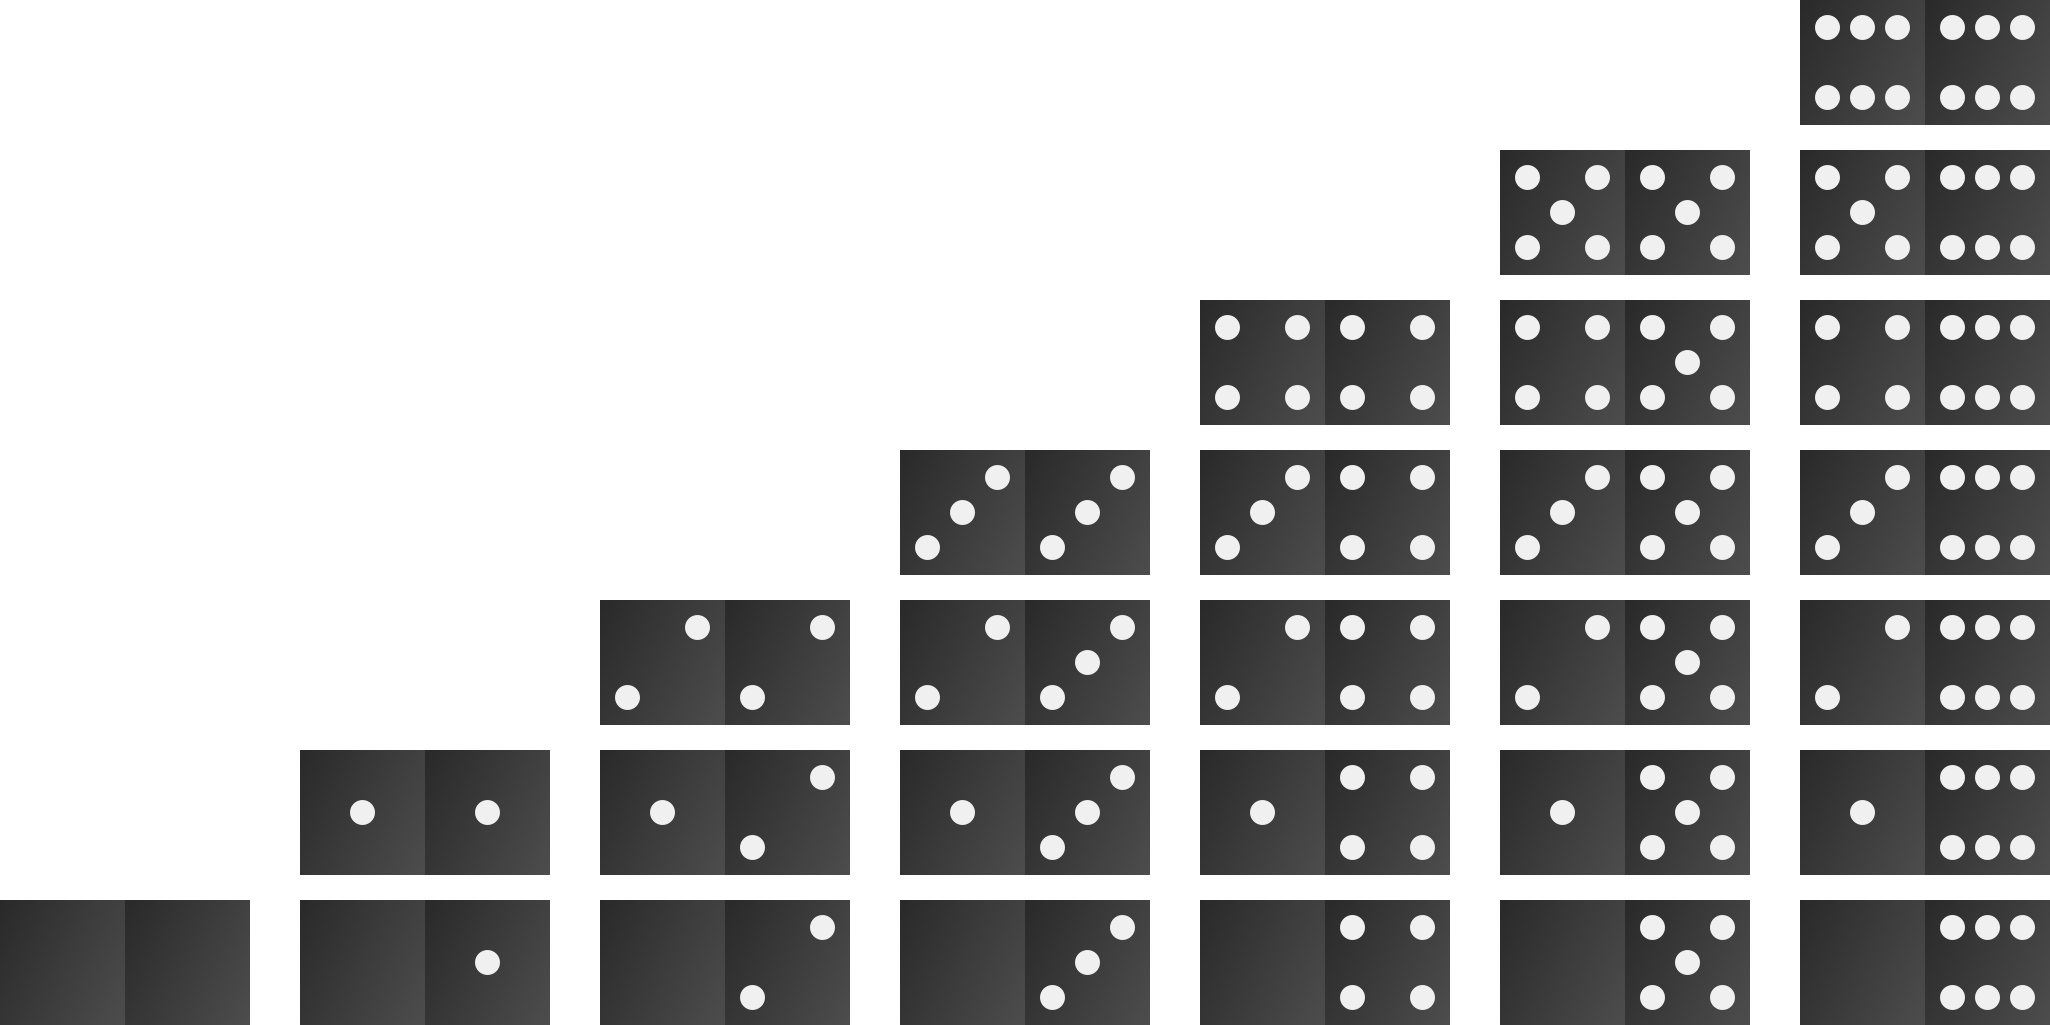
\includegraphics[width=0.65\linewidth]{img/dominomatrix.png}
  \caption{A so called ‘double-six’ domino set with which is the most common variant of dominoes is played.}
  \label{fig:dom_set}
\end{figure}

In its simplest form, dominoes is a two player game with complete information as all tiles are equally distributed between the players. The rules for this simple variant are detailed in Appendix \ref{a:domrules}.

Even this simple variant however maintains a comparably high mathematical complexity. For the case of two players, the number of possible starting states $n_{ss}$ for a game where all domino tiles are divided up equally between players are all possible combinations of all dominoes on the players’ hands:

\[n_{ss} = \binom{n}{\frac{n}{2}} \textrm{with $n$ being the set size.} \] 

This means that for the ‘double-six’ variant shown above with only two players there over 40 million starting states. The ‘double-three’ variant in contrast only has 252. 

The complexity of a game is also determined by its branching factor, the average number of available moves from a position. For dominoes this is hard to specify as it involves the number of dominoes in a player’s hand and the number of places that domino can be positioned on the board. If the domino can be placed in more than one location, depending on the domino and the player’s strategy, the branching factor can increase up to a factor of 4.

Dominoes therefore is a sufficiently complex problem, providing an appropriately challenging basis for any project trying to derive winning strategies for this game. 


\subsection{Why Reinforcement Learning?}
\label{sec:rl}
Due to it’s comparably high complexity, trying to find good strategies for dominoes is a problem to which the common supervised machine learning approaches cannot offer a satisfying solution. Supervised Learning (SL) is when an agent is given training data, consisting of input-output pairs and learns a function that approximates the underlying relationship between inputs and outputs  \citep{russell_artificial_2010}. With regards to game playing, two obvious problems arise with this approach: first, for training expansive data sets are needed that indicate to the agent which moves are good and which are not. However, from only observing and never actually playing games, the agent will not develop its own strategy but will learn the strategies used to generate the training data. Secondly, while SL assumes all learning samples to be independent, this is not the case with data sampled from sequential games. Instead these samples are highly correlated as one state follows the next. 

These constraints however do not apply to Reinforcement Learning (RL). In RL, the agent interacts with an environment and - instead of true labels - learns from reinforcement signals (rewards or penalties) following its actions. In the case of dominoes the agent would be penalised if they did an invalid action and would be rewarded or penalised by finishing a game (-1 for a loss and 1 for a win). Generally the agent would therefore try to minimise penalties and maximise the reward. However, in many games - as well as in dominoes - rewards do not occur at every time step and instead are mostly received at the end of an episode. This makes them sparse, delayed and noisy \citep{mnih_playing_2013} and increases the difficulty of the learning task as the agent has to deduce with action led to the reward \citep{francois-lavet_introduction_2018}.

Still, intensive RL research has been able to overcome these limitations - especially with regards to games, which often provide a highly predictable and thus suitable framework for an agent to freely explore. There have been many other successful and well publicised RL implementations for all kinds of games \citep{wiering_reinforcement_2012} which motivated us to gather experience with this machine learning paradigm.


\section{Project Execution}
\subsection{Problem Formalisation}
\subsubsection{Game Description Language (GDL) and Answer Set Programming (ASP)}
Before being able to learn winning strategies for dominoes, we first had to find a way of representing the rules of the game in a way that allowed automatic evaluation of possible moves and rewards. As mentioned section 1.3., declarative programming is a possible way of formalising such rules.

Game Description Language (GDL), also called Game Definition Language by \citet{love_general_2008} is a declarative logic programming language which formalises the state of a game as a series of facts and the game mechanics as logical rules. It provides game independent relation constants to describe the dynamics of any game. In this project, some of these constants are of special interest:
\begin{itemize}
\setlength\itemsep{0.01em}
  \item role(r) means that r is a role in the game, this usually refers to players
  \item init(d) means that the datum d is true in the initial state
  \item true(d) means that the datum d is true in the current state
  \item does(r,a) means that player with role r performs action <a> in the current state
  \item next(d) means that the datum d is true in the next state
  \item legal(r,a) means it is legal for r to perform action a in the current state
  \item goal(r,v) means that player with role r would receive the utility with  value v in the current state, should the game terminate in this state
  \item terminal means that the current state is a terminal state
\end{itemize}

Now, based on an encoding using these formalisms, a logical solver can compute all sets of facts that are true for the initial state. Given that initial state and the players’ actions it also allows to compute the set of facts true in the follow-up states of the game, including if that state is terminal (and the associated reward values for each player) and (in case the state is not terminal) the set of legal moves for a player \citep{love_general_2008}.

To actually calculate the set of true facts for any given game state, we use the clingo ASP system developed by the Potassco research group at Uni Potsdam \citet{gebser_clingo_2014}. ASP is a form of declarative programming oriented towards difficult, primarily NP-hard, search problems \citet{lifschitz_answer_2019}. Clingo is made up of gringo (a combination grounder) and clasp (a solver) which in combination first reduce the encoding to a set of logical statements and then solve it based on deduction as failure. 

\subsubsection{Game Encoding and Vector Representation for Dominoes}
\label{sec:game_encoding}
In summary, we use constructions from the GDL formalism to encode the game rules of dominoes in ASP.
We decided to limit the game complexity from the start by only allowing a total of ten tiles with numbers from zero to three on them. Since in our version of the game dominoes can only be placed at the free ends of the existing chain of dominoes and all dominoes are divided up between the two players, the game can be fully summarised by keeping track of which dominoes are held by each player (dominoes which are not held by either player are somewhere in the chain), the numbers at the ends of the chain, and an indication of which player’s turn it is. As GDL is an open language, its vocabulary can be extended. We used this property to encode this additional information specific to the game dominoes:

\begin{itemize}
\setlength\itemsep{0.01em}
  \item To represent the current number on the stack, we add the constants stack(l) and stack(r)
  \item The constant in\_hand(X,D) keeps track, which domino D is held by which player X
  \item The constant control(X) indicate which player’s tun it is
\end{itemize}

These facts can then be translated in a one hot encoded vector of length $2n+2(m+1)+2$ representing the current board with both the players hands, the numbers at the end of the chain and which actor is currently in control. An action can be similarly displayed as a vector of length $2n+1$: each domino can be placed either to the left or to the right ($2n$), and if no domino can be placed, only one possible action remains: passing. 
Figure \ref{fig:encoding} shows an example of the final encoding used in our project for a transition between states for our 3-by-3 domino game.

\begin{figure}
  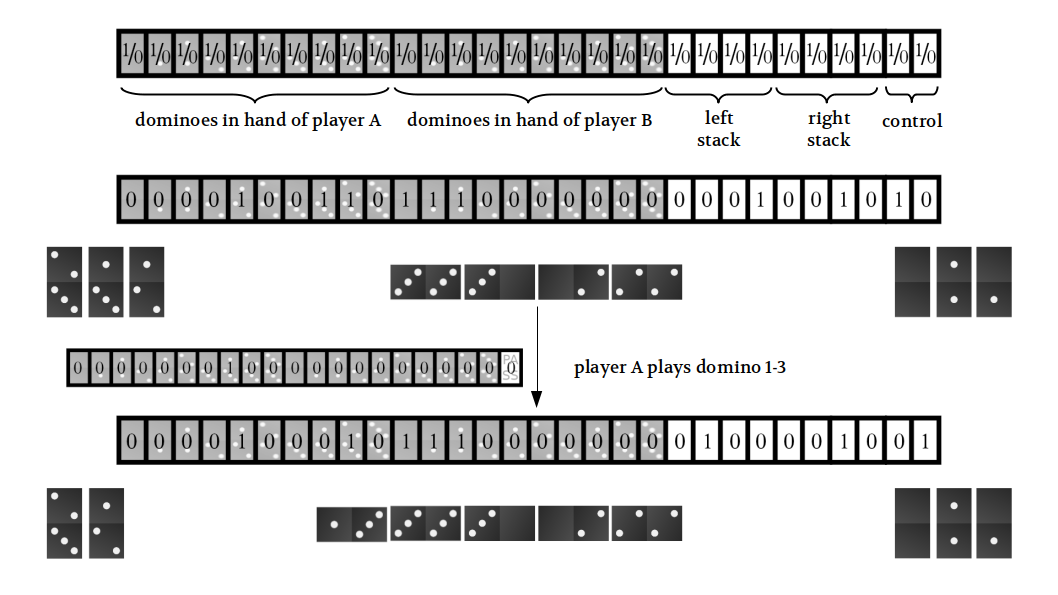
\includegraphics[width=\linewidth]{img/encoding.png}
  \caption{An arbitrary game state and a transition following an action represented visually and with their corresponding one-hot-encoded vectors.}
  \label{fig:encoding}
\end{figure}

\subsection{Application of Q-Learning}
\subsubsection{Algorithm Selection}
\textbf{Basic concepts of Reinforcement Learning.}
Before detailing our specific approach, it seems reasonable to recall the key concepts in Reinforcement Learning (RL). As discussed in section \ref{sec:rl}, Reinforcement Learning describes a formal framework for the machine learning of sequential decision making \citep{francois-lavet_introduction_2018}. Its core concept is the interaction of an artificial agent with a given environment. This process is called a Markov Decision Process which is pictured in Figure \ref{fig:mdp}. In our case, the agent interacts with the representation of the domino game (all dominoes in both players' hands, in the chain on the board and the numbers on both sides of the stack).

\begin{figure}
  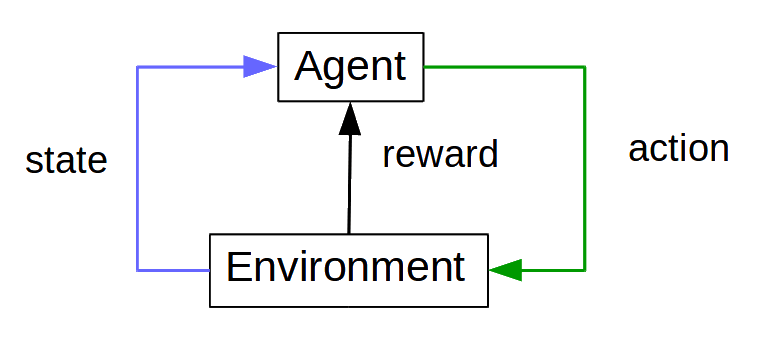
\includegraphics[width=8cm]{img/mdp.png}
  \centering 
  \caption{General depiction of a Markov Decision Process in which an agent interacts with an environment through actions based on a state observed in the environment. The environment also provides a reward to the agent.}
  \label{fig:mdp}
 
\end{figure}

At each (time)step $t$ of the interaction the agent can observe the state $s_t$ of the environment. Based on this observation of the state, the agents can then decide on a possible action $a_t$ to take. The set of all valid actions is often referred to as the action space. Performing an action $a_t$ changes the state from $s_t$ to $s_{t+1}$. The sequence of states and actions is called a trajectory $\tau = (s_0, a_0, s_1, a_1, …)$. For our specific dominoes encoding, the agent always observes the entire state with no omitted information and can decide to play any domino on their hand or pass. The agent’s discrete action space is solely defined by the current state: dominoes can only be placed if they include a number on top of either side of the stack and a pass is only and exclusively in the action space when no domino can be placed. 
For each action, the agent receives a reward $r_t$ which is generated from a reward function $R(s_t, a_t)$. In the case of dominoes the reward signal is spare as the agent is only rewarded at the end of the game (either $1$ or $-1$ for winning and losing respectively) and thus the reward for most steps will be $0$. 

The overall goal of the agent is to maximise the cumulative reward over the trajectory $\tau$ which is the expected return of rewards for a given trajectory. In our specific case, it is the agent’s goal to get to $R(\tau)$ as close to one as possible. 

The function used by the agent to decide which action to take given a specific state is called the policy $\pi$. The estimate for the expected reward in a given state or for a given state-action pair (on which the policy acts) is determined by a value function $V$ (or action-value function $Q$) which is always dependent on the agent's policy.
\\ 
\\
\noindent \textbf{Choosing an appropriate RL algorithm.} Having recapped the basic theory of Reinforcement Learning, we had to choose an algorithm that would fit our dominoes implementation. We wanted the algorithm to learn dominoes without having a model of the environment. This way we wanted to investigate if it would be able to learn the rules (meaning which actions are valid in what states) as well as a good strategy just from experience. We therefore decided to use a model-free over a model-based approach, that would assume that the agent has access to a model of the environment \citep{russell_artificial_2010}.

Model free RL algorithms can be further differentiated into on-policy and off-policy algorithms. On-policy algorithms start with a given policy and sample the state space based on this policy to improve the policy. The same policy that is used for control is also approximated at the same time. Off-policy algorithms on the other hand use two policies: one policy used to generate behaviour (behaviour policy) and the policy that is learned about and becomes the optimal policy (estimation policy) \citep{sutton_reinforcement_2018}. As our environment is deterministic and has a finite, discrete action space, there should be one optimal action for a given state. Based on this fact, we decided to use off-policy methods as it allows for a deterministic estimation policy while at the same time incorporating a non-deterministic behaviour policy that keeps sampling from all possible actions.

After considering our problem and possible approaches, we eventually decided on the DQN (Deep Q-Network) approach that combines off-policy Q-learning with deep neural networks and will be explained in more detail in the following section.
\\ 
\\
\noindent \textbf{Q-Learning and the Deep Q-Network.}
For any reinforcement learning setting, we can consider a policy $\pi$ to be better than another policy $\pi’$ if the expected return for each possible state-action pair $q$ given $\pi$ is greater than the expected return given $\pi’$. To estimate the expected return for a given state action pair, we use an action-value function $Q^{\pi}(s,a)$. It defines expected return for a state action under policy $\pi$.
\[ 
 Q^{\pi}(s,a) = E\left[  \sum_{k=0}^{\infty}  \gamma^k R_{t+k+1} \right]
\]

The function $Q^*(s,a)$ defines the expected return for a state action pair under the optimal policy $Q^*$. $Q^*$, by definition, will always lead to the maximum return achievable by any policy $\pi$ for each state action pair. The goal of Q learning is therefore to approximate $Q^*$ as good as possible by learning the optimal q-values for each state action pair. $Q^*$ obeys the Bellmann optimality equation which guarantees self-consistency: it states that the value of a state $s$ is the reward received in that state plus the discounted reward of the next state $s’$ when the optimal action is chosen.
\[ 
 Q^*(s,a) = E\left[  R_{t+k+1} +  \gamma max Q^*(s',a') \right]
\]
In order to make sure that the agent can actually find the optimal behaviour, it needs to strike a good balance between exploring the environment (by choosing random moves) and exploiting the environment (by choosing the move that maximises the expected return). It seems reasonable that the agent should explore the environment first to gather information and only later use the given information to derive an appropriate policy. In Q learning this behaviour can be achieved with an epsilon-greedy policy, which defines an exploration factor $\epsilon$ that determines the probability of the agent exploring a given environment. $\epsilon$ is initialised with $1$, forcing the agent to initially explore the environment. Then, at each time step, a random number $r$ between 0 and 1 is generated. If $r < \epsilon$, the agent will move randomly; if $r \geq \epsilon$ however, the agent will greedily choose the action with the maximum Q value. To make sure that exploratory behavior decreases over time, epsilon will decay at some preset rate yielding a decreasing probability of exploration.

Given these assumptions, we could estimate the optimal value function $Q^*$ by iteratively updating $Q_i \rightarrow Q_{i+1}$. This process is commonly referred to as value iteration and $Q_i \rightarrow Q^*$ as $i \rightarrow \infty$. However, this theoretical approach is rather impractical when applied practically for two main reasons: First, the bigger the state space as well as the action space, the more updates are necessary to approximate $Q^*$ to a satisfactory degree. Also, as the Q function is separately estimated for each sequence, it does not generalise well to other sequences. 

To address this issue, we use a function approximator in order to estimate $Q^*(s,a) ~ Q^*(s,a, \theta)$. This approach is commonly called Q-learning. Mnih et al. (2013) combined Q-learning and neural networks into the Deep Q-Network approach in which the function parameters $\theta$ are approximated using the weights of a neural network. For training, they use a technique called experience replay: the agent’s experience tuples at time $t$ $e_t = (s_t, a_t, r_{t+1}, s_{t+1})$ are collected in a set named replay memory. Experience replay is the act of learning by randomly sampling from replay memory. This provides data efficiency as every experience at any time can be used for training and, more importantly, breaks up the correlation between different samples thereby reducing update variance. 

The network’s loss is calculated by comparing the Q-value outputted by the network for the action in the experience tuple  and the corresponding optimal Q-value, or target Q-value, for the same action. The loss can therefore simply be expressed as
$$\begin{aligned}
Q^*(s,a) - Q(s,a) = l\\
 E\left[  R_{t+k+1} +  \gamma max Q^*(s',a') \right] - E\left[  \sum_{k=0}^{\infty}  \gamma^k R_{t+k+1} \right] = l
 \end{aligned}$$
However, the challenge is to calculate the target Q-value Q* for all actions. As target Q-value is calculated using the Bellman equation shown above, in order to calculate the maximum Q*-value, we need to additionally pass the follow up state s’ to the network. This way we can calculate the maximum Q*-value for the next state which we can use to approximate Q* for the current state. This effectively boils down to two subsequent forward passes through the network before a gradient can be obtained. 
 \citep{russell_artificial_2010}.


\subsubsection{Implementation}
We implemented a DQN-Agent with Epsilon-greedy policy, $\epsilon = .1$, using the keras-rl2 library and a three-layer network architecture. Our specific structure consisted of 120,30, and 120 neurons on the respective layers. We additionally used random initial states as we did not want the agent to overfit to a specific board configuration but generally learn the game of dominoes. Furthermore, we penalised invalid moves with a reward of -100 and ended the current episode. Through this strong penalty, we expected the agent to quickly extract which moves were legal in what situation and which moves were not. We also considered that the opponent’s behaviour could have an effect on the agents learning, which is why we let the agent play for 5000 iterations, either against a random player or against a strategic player who would always play the tile that minimised the options for the other player.

\subsubsection{Benchmarking and results}
For benchmarking we used 10 different initial states. After 1000 iterations of training, the agents would play 100 games against a random player in each initial state yielding a total of 1000 games. A random player was used for benchmarking as it symbolised the lowest possible benchmark and thus gives a good indication to what extent basic learning takes place at all.

\begin{figure}
  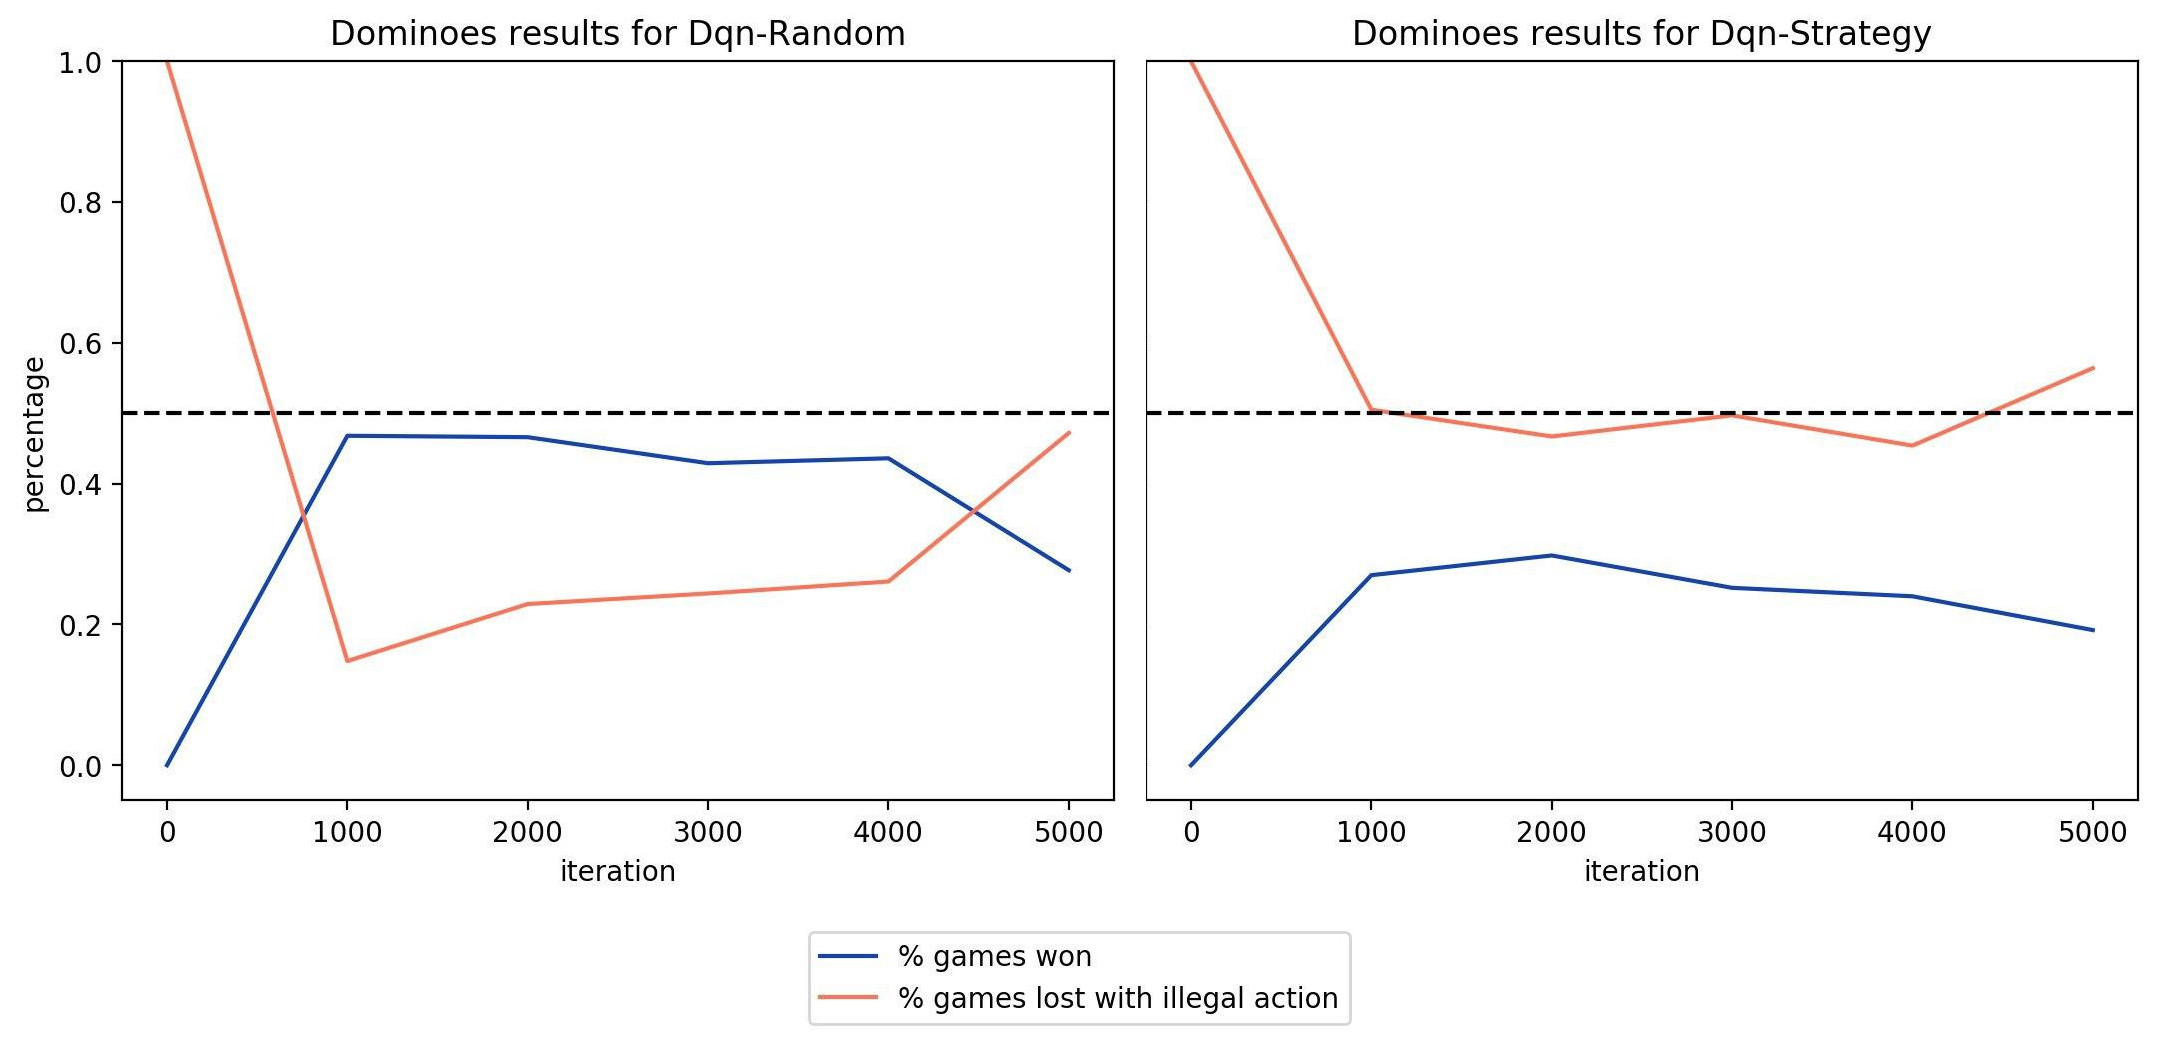
\includegraphics[width=\linewidth]{img/dqn_both.jpg}
  \centering 
  \caption{Benchmarking results for DQN agents trained against a random and a strategic player. Benchmarking was performed every 1000 training iterations and the percentages of games won and games lost with an illegal action were recorded.}
  \label{fig:dqn_both}
\end{figure}

Figure \ref{fig:dqn_both} shows the results for both agents. It becomes clear from neither of the blue lines crossing the 50\% threshold that both networks perform rather poorly and are not able to consistently beat a random player.
Interestingly, the model trained against a random player wins a greater percentage of matches. This might be because of the opponent’s behaviour during training: A random opponent will not choose moves systematically and thus positively contributes to exploring the state space as the agent will experience more of the overall game. A strategic opponent on the other hand will always act according to a certain strategy which also limits the agents capability to learn.

The model trained against the random opponent is also more effective in representing some of the game dynamics. This becomes clear by the rapidly declining fraction of illegal moves between the first and second benchmark. However, as the training goes on, the model seems to unlearn some of the represented knowledge as the percentage of illegal moves starts to rise again.

Generally, while some learning seems to have taken place, the results are far from satisfactory. Both models cannot beat a random player and fail to represent the entirety of game dynamics which is indicated by the puzzling increase of losses due to illegal moves over more training time.

\subsubsection{Resulting project modifications}
Based on these disappointing results, we considered in what direction we would take the project. We had two propositions on why the model did not learn: Firstly, the model architecture used was not complex enough to capture the game’s actual complexity. However, this train of thought did not turn out to be promising. We tried expanding the network on a small scale but these expansions did not have an effect and as we were not sure on how to go about constructing a more complex architecture that could be better suited to the given task, we decided to not pursue this further. Secondly, we could see that the algorithm did not seem able to completely represent the game dynamics, consistently choosing moves that were not legal.

We therefore decided to modify our approach. We would abandon further testing of the DQN and instead return to supervised learning to see if knowledge of the game dynamics would lead to an improvement in estimating an action’s expected value. We also decided to test the popular AlphaGo Zero algorithm as this would solve the problem of selecting an opponent for the agent through self-play. 

This development further warranted the abandonment of pre-implemented RL libraries. Instead we chose to create our own framework that allowed for various approaches to be applied to any game encoding. Another feature of this framework would be game visualisation in order for us to see beyond the aggregated benchmarking results and to more clearly identify conceptual advances if we observed any.


\subsection{Application of Deep Supervised Transfer Learning}
\subsubsection{Deep Supervised Transfer Learning}
The core idea of transfer learning is to improve learning on a target task by using the knowledge gained in a previously learned source task \citep{olivas_transfer_2010}. It is commonly used in deep learning, especially with regard to computer vision. The underlying assumption is that the early layers of a deep neural network encode more generic features whereas later layers are more specific to the dataset it was trained with. This is why in order to use transfer learning with a neural network one usually fixes the weights of all but the top layer(s) of a neural network that is already trained on a source task. Then the output layer is adapted to fit the specific task and 'fine-tuned' using a new training dataset for the target task. Figure \ref{fig:trnsfr_bttr} shows how transfer learning commonly improves learning the source task: it can either improve the initial performance on the target task (indicated by a higher intercept), the time it takes to fully learn the target task (indicated by a higher slope), or improve the overall performance (indicated by a higher asymptote).

\begin{figure}
  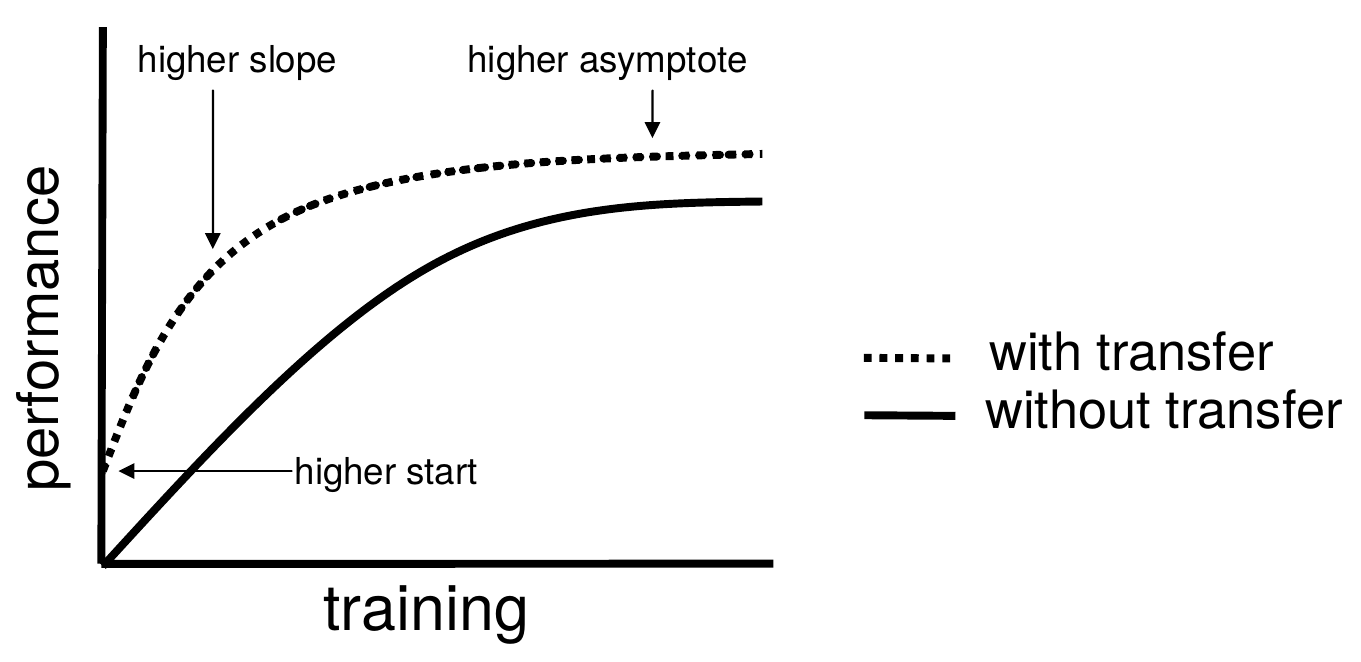
\includegraphics[width=10cm]{img/trnsfr_bttr.png}
  \centering 
  \caption{Three common ways in which learning a target task can benefit from a previously learned source task as shown in \citet{olivas_transfer_2010}}
  \label{fig:trnsfr_bttr}
\end{figure}

Applied to our specific problem, we wanted to employ transfer learning in order to answer two questions: Is a simple neural network able to learn the game dynamics of dominoes? And does the knowledge gained through understanding the game dynamics (source task) help the neural network to approximate which state action pairs are more likely to result in better moves (target task)?

\subsubsection{Data Generation with Monte Carlo Tree Search}
Abandoning RL methods and refocusing on Supervised Learning (SL) brought with it the challenges common to all SL approaches: coming up with a sufficiently sized data set to learn with. The data we needed would need to include a state-action pair, the follow-up state as well as some measurement that roughly corresponds to the expected value of that specific state action pair. Fortunately enough, we had already started looking into the Alpha Zero algorithm used by \citet{silver_mastering_2017} which featured Monte Carlo Tree Search (MCTS). 

MCTS is method  for finding  optimal  decisions  in  a  given  domain  by taking random samples in the decision space and building a search tree according to the results \citep{browne_survey_2012}. We can apply this framework to the field of sequential games if we conceptualise every game state as a node in the search tree linked to follow-up states by the possible actions that can be taken in that state. The tree is usually constructed in four stages that are also shown in Figure \ref{fig:mcts}. During node selection the algorithm traverses the tree starting from the root node. It chooses the node on the next level by comparing the Upper Confidence Bound 1 ($UCB1$) score of each child node. The UCB1 is calculated as follows

$$UCB1 = \frac{v}{n} + C \sqrt(ln \frac{N}{n})$$

In the above calculation $C$ is the exploration/exploitation factor (usually 2), $N$ are the number of times the parent node has been visited, $n$ are the number of times this node has been visited and $v$ is the estimated value of that node. By always choosing the child node that maximises the $UCB1$ score the algorithm automatically balances exploration and exploration as the right hand term will be greater for nodes that have not been visited (as often). On the other hand, the higher the estimated value for that node the higher is the incentive for exploitation. If all nodes have the same $UCB1$ score, one node is chosen at random. 

After having reached a terminal node, the algorithm checks if this node has been previously visited. If it has been, the node will be expanded and a new layer with all possible follow up states as nodes will be created. If it has not yet been visited, a simulation will be performed according to a default policy. In our case, a complete game of dominoes between two random players will be played from this stage and the result of that match will be the new estimated value for that node (if the node is terminal, then the actual result of the game will be used as value). This information is then back propagated through the tree adjusting the visit count as well as the estimated value for the nodes on the path. The estimated value for the parent nodes in our case is the total value of all the nodes child nodes. This process can be repeated until most of the search tree is traversed, time runs out or a fairly stable solution is reached.

\begin{figure}
  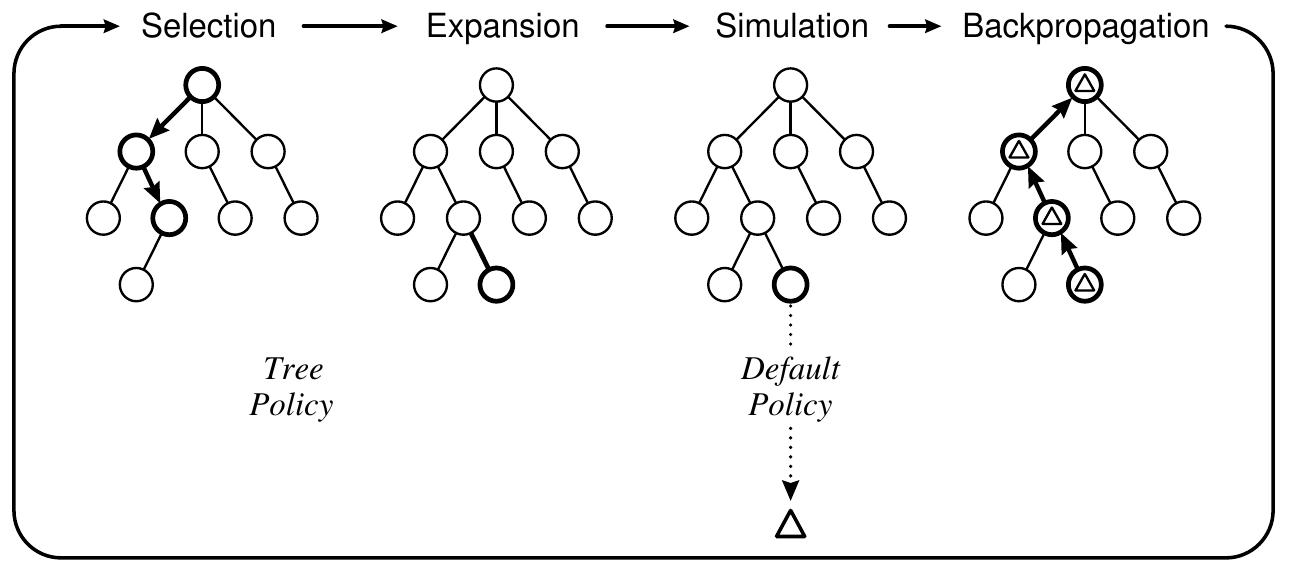
\includegraphics[width=\linewidth]{img/mcts.png}
  \centering 
  \caption{ One iteration of the Monte Carlo Tree Search algorithm as shown in \citet{browne_survey_2012}}
  \label{fig:mcts}
\end{figure}

This way the MCTS algorithm builds a search tree in asymmetric fashion. Due to the weighting of exploration and exploitation, the algorithm will generally prefer nodes that have a higher expected value and thus lead to winning the game with a greater probability. Both probability and expected value thereby serve as good estimates of how “good” a state (and thereby the action leading to it) is. This process works without domain knowledge and is very flexible with regards to the number of times it is being run, which made it a very good fit for our issue of data generation.

We decided to run 1000 iterations of the MCTS from 200 different initial states. This resulted in more than 11500 training tuples, containing a state and an action, encoded as described in section \ref{sec:game_encoding}, the follow up state and the corresponding probability of the MCTS algorithm visiting that state ($p = \frac{n}{N}$). Due to the nature of the algorithm described above we used this probability as an adequate measure connected to move quality.

It is worth noting that we were not able to use all collected training tuples in the training as some encodings repeated themselves. This is most likely because our encoding does not track the history of the game by representing the entire board but only provides aggregate information about which stones are on the table and what the number of eyes on each stack is. This way it is possible that from different starting states, game states were reached that were different in their history but shared the same encoding. These duplicates could not be used for training as the same input would lead to different output labels which is why we removed all states that had been visited less than the duplicate with the maximum number of visits. This yielded a final training data set with 6367 tuples, 10\% of which were used for testing.

\subsubsection{Model Setup}
We used a similar model to the one employed in the DQN but with the input and output layer adjusted to match the source learning task. This resulted in a three layer structure with 51 neurons in the input, 120 neurons in the hidden, and 30 neurons in the output layer. Additionally L2-regularisation was added on the medium layer and dropout was used before the last layer. A one-hot encoded vector representing a state (length 30) and an action taken in that state (length 21) was used as input. The output would be another one-hot encoded vector with length 30 that encoded the follow up state. Naturally the loss for a one-hot encoded vector was chosen to be categorical cross entropy. The optimiser used for the source task was Adam.

For the target task we used the same architecture as in the source task and only changed the output layer to predict a single value - the probability returned by the MCTS algorithm. The distribution of labels is displayed in Figure \ref{fig:hist_labels}. It is clear that the labels are not equally distributed. This makes sense however, as most actions have a low probability of success. The two other main peaks occur for ambiguous actions ($p \sim 0.5$) and actions with a high probability of winning. Binary cross entropy was used as a loss function for this target task.

\begin{figure}
  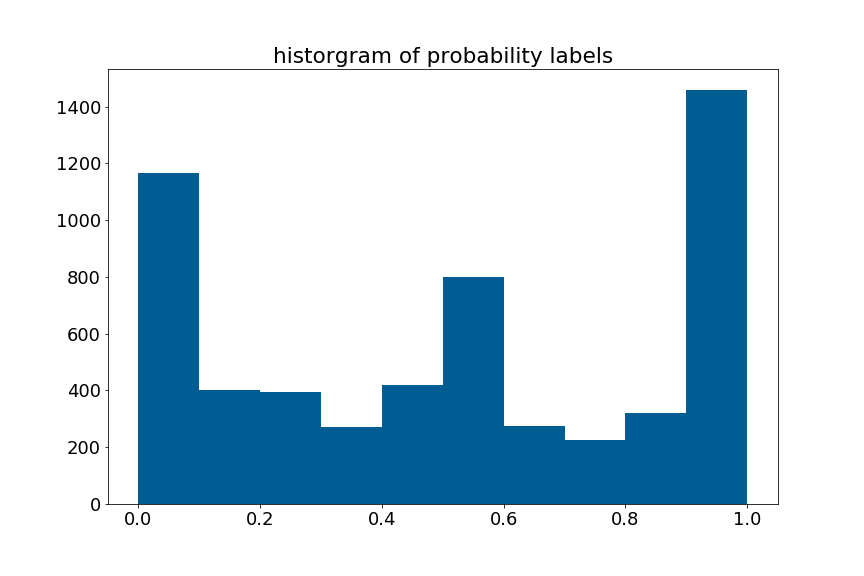
\includegraphics[width=10cm]{img/hist_labels.png}
  \centering 
  \caption{Histogram of move probabilities obtained via Monte Carlo Tree Search}
  \label{fig:hist_labels}
\end{figure}

As we were unsure about the best configuration of hyper parameters, we ran a grid search with nested three-fold cross validation to pick the best combination. We searched over different values for learning rate (0.0001, 0.001, 0.01), batch size (10, 50, 100, 500), and regularisation term (0.01, 0.001, 0.0001) and used the opportunity to test the effect of two additional factors: transfer learning as well as model depth. Transfer learning meant that we would re-train the previous model with a fixed second layer while the model would just be initialised with random weights in the non-transfer learning condition. The model depth condition differed between the original three-layer model and a five-layer model to which an additional two layers (120 and 250 neurons) were added before the output layer. This resulted in 114 different combinations of parameters with three times the number of models trained due to the cross validation.

\subsubsection{Benchmarking and Results}
Figure \ref{fig:src_tsk} shows the results for the source task, the learning of the game dynamics. It becomes very clear through the steep decline of the loss curve and the quickly rising accuracy score that the network is quickly able to extract the relevant information and to produce the correct state as a result. We can also see that the testing loss is even smaller than the training loss which would usually be a sign of overfitting to the dataset. In our case however, overfitting to the dataset is desirable behaviour as it means that the algorithm has understood the deterministic dynamics of dominoes. 

\begin{figure}
  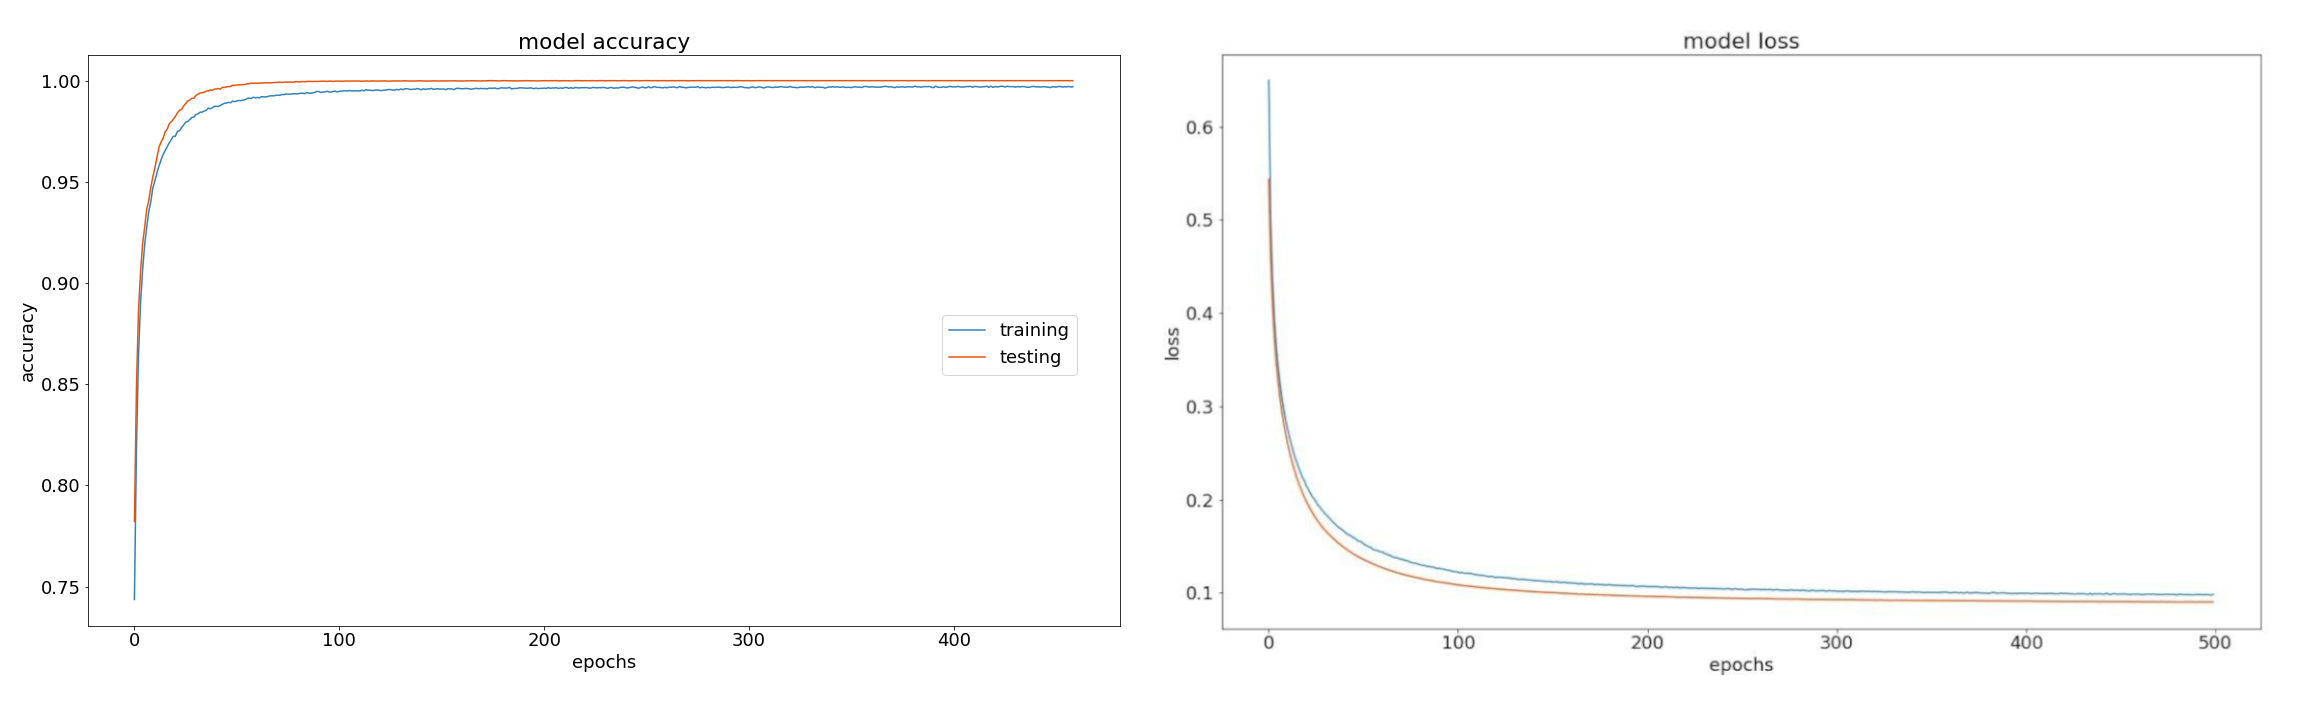
\includegraphics[width=15cm]{img/src_tsk.png}
  \centering 
  \caption{Accuracy and loss curves for the source task of learning the game dynamics of through one-hot encoded state and action vectors.}
  \label{fig:src_tsk}
\end{figure}

To first take a descriptive look at the effects of transfer learning to see if any of the indications of a positive effect of transfer learning could be observed, we chose the model for which both versions - with and without transfer learning - ranked highest when sorting the trained models by mean loss over all folds in ascending fashion. The model fulfilling these criteria had three layers and used a batch size of 100, a learning rate of 0.001, and a regularisation penalty of 0.0001. The results are shown in Figure \ref{fig:trnsfr_both}. The model with the smallest loss was additionally selected for benchmarking but lost all games through illegal actions.

\begin{figure}
  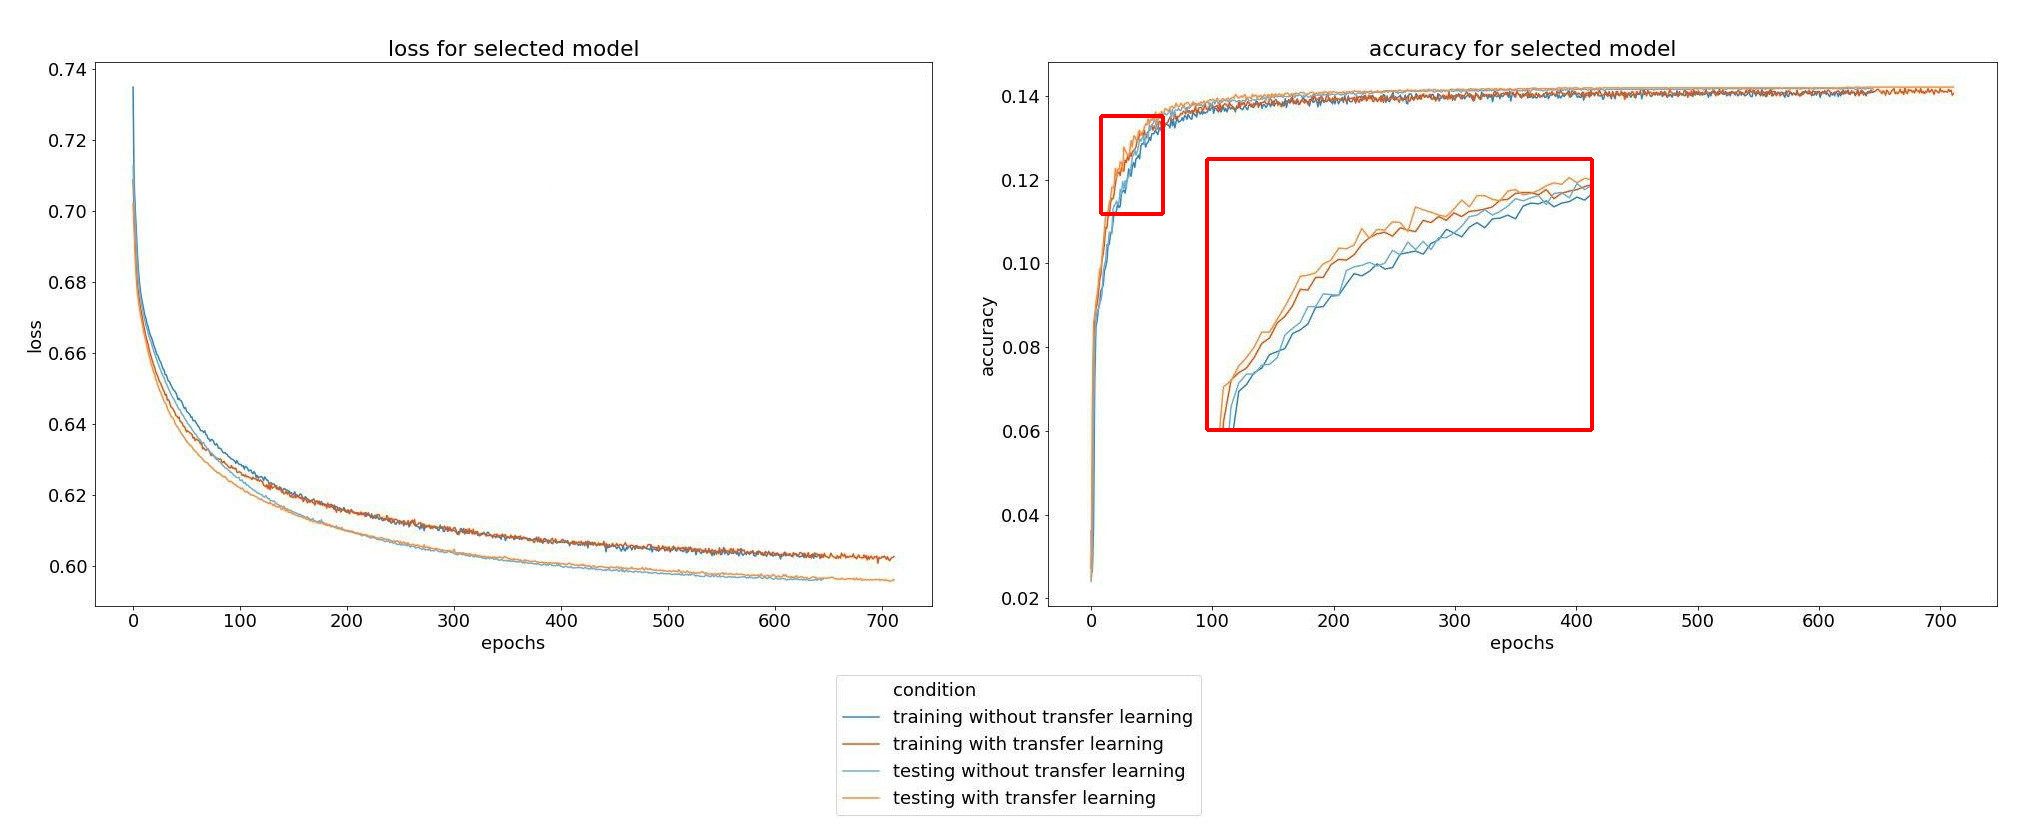
\includegraphics[width=15cm]{img/trsnfr_both.jpg}
  \centering 
  \caption{Accuracy and loss curves of a selected model for the target task predicting move probability through one-hot encoded state and action vectors. The area surrounded by the red border inside the accuracy graph is a zoomed-in view of the first 50 iterations.
}
  \label{fig:trnsfr_both}
\end{figure}

We can see that both loss and accuracy are significantly worse than in the source task. We also do not see great differences between the models with or without transfer learning. However, when zooming into the accuracy curve, we can indeed observe a steeper slope for the conditions of transfer learning, which relative to the overall performance is still negligible but at least shows some correspondence with previous literature.

To get a better overview of the different performance for the different combinations, we wanted to group the data by the factors of interest, meaning transfer learning and model depth and therefore average over all learning rates, batch sizes, and regularisation penalties. To do so however, we first have to check if this step is justified by examining the mean loss for batch sizes and learning rates in order to check if the mean accurately approximates the mean over all conditions. The results displayed in Figure \ref{fig:means_aggr} show some minor but negligible differences for the mean loss between different batch sizes and learning rates. The same is true for the different regularisation parameters.

\begin{figure}
  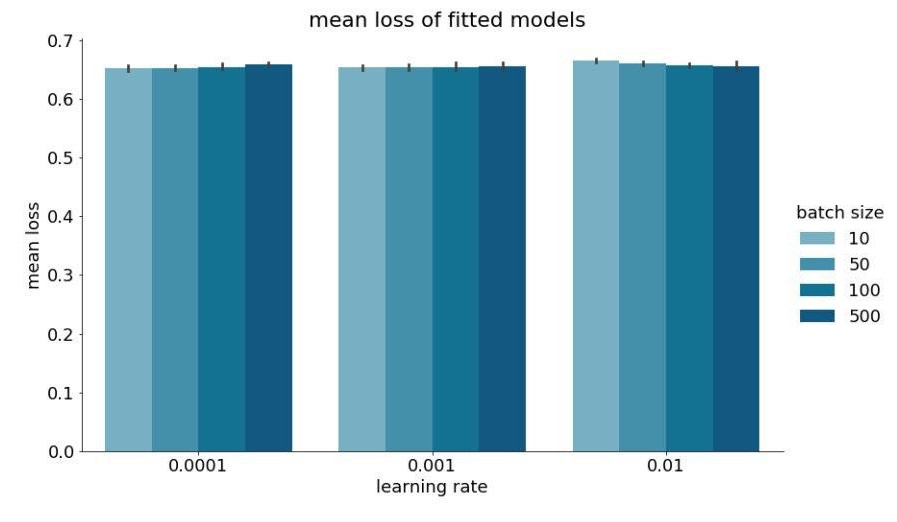
\includegraphics[width=8cm]{img/means_aggr.jpg}
  \centering 
  \caption{Mean loss for models with different batch sizes and learning rates.}
  \label{fig:means_aggr}
\end{figure}

Being able to average the data over the conditions revealed interesting findings which are displayed in Figure \ref{fig:grdsrch}. We can see that on the aggregated level, transfer learning does not seem to have a significant effect on performance - this is also not affected by a deeper network. This leads to the conclusion that the model either was still not complex enough or - more likely - that not enough training data was available for this significantly more complex target task. Curiously the time needed for the models to reach a stable solution is significantly smaller for deepened networks (early stopping was used after 50 iterations with a minimum delta of 0.0005). This is most likely due to the advantage in parameter numbers which allow for more and faster storage of information.

\begin{figure}
  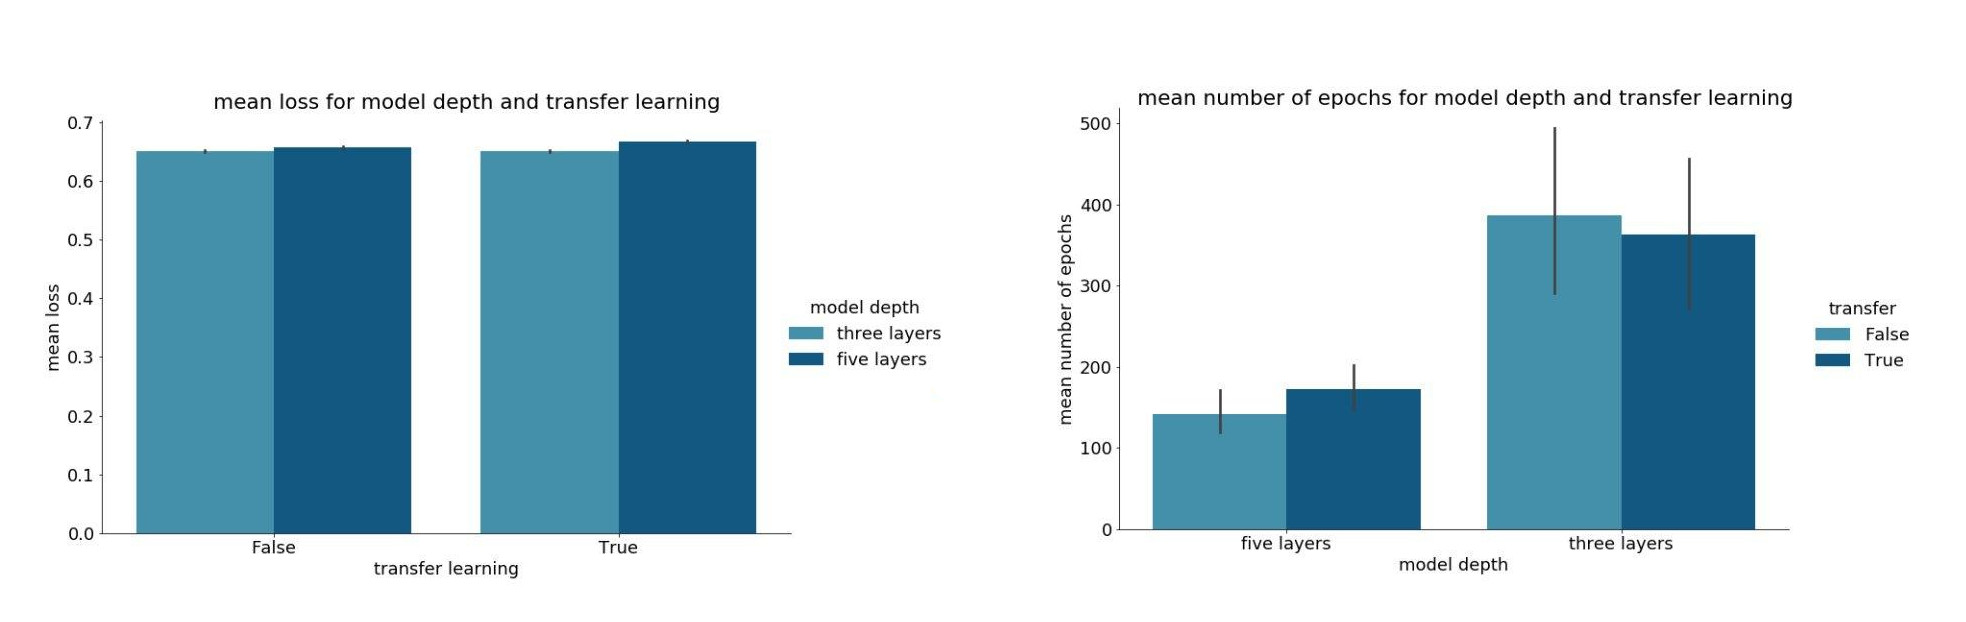
\includegraphics[width=\linewidth]{img/gridsrch_comb.jpg}
  \centering 
  \caption{Mean loss and mean number of epochs of the models fitted in the grid search aggregated over the factors transfer learning and model depth.}
  \label{fig:grdsrch}
\end{figure}

\subsubsection{Discussion}
While the results brought to light some interesting results concerning the relationship of model depth and fitting speed, the actual goal of creating a model that could appropriately represent not just the game dynamics but also a strategy of playing dominoes was not met. 

A possible reason for this result is the lack of sufficient training data which was due to information shortages in the state encodings. The argument that the model was not sufficiently complex does not hold, since more complex and deep models did not significantly improve performance. Looking back, it might have been a good idea utilise the entire data generated by the MCTS, also including the estimated value instead of predicting just the probability, which is high not just for good moves but also for moves without alternatives.

Overall the results are far from optimal and show that Supervised Learning might not be the method of choice for tackling the learning of game mechanics and strategies. This is why, with our last approach we returned into the realm of Reinforcement Learning, attempting to apply the famous AlphaGo Zero algorithm to our problem.

\subsection{Implementation of AlphaGo}
\subsubsection{The AlphaGo Zero algorithm}
AlphaGo Zero is based on the original AlphaGo algorithm developed by \citet{silver_mastering_2017} which used two neural networks to learn the game Go: A convolutional policy network outputting move probabilities, which was initially trained through supervised learning to predict expert moves, refined by policy gradient reinforcement learning, and a value network for state evaluation. This second network was trained to predict the winner of games of self-play by the policy network. After training, both networks were combined with MCTS into a lookahead search with the policy network being used to narrow the search tree. This algorithm defeated Fan Hui, the European Go champion, in 2015 and a slightly altered approach defeated Lee Sedol, holder of 18 international titles, in 2016. While being very successful at beating human players, the original AlphaGo algorithm still had a few issues: it was still based on human data for (supervised) learning and used two separate networks to predict move probabilities and values. 

AlphaGo Zero addresses these issues by training only one network and doing so only through self play, which means that there is no need for human knowledge within the algorithm. It uses a deep convolutional neural network $f_\theta$ with parameters theta. As input it takes a state $s$ and its history and outputs move probabilities of selecting each move $P(s,a)$ and value $V_\theta$, an estimate of the current player winning from the current state. 

The training of AlphaGo Zero can be divided into three parts: First, \emph{self play} which is illustrated in Figure \ref{fig:selfplay}. At the start the model is initialised with random weights and then starts playing against itself. In each state $f_{theta}$ is used to estimate the policy, meaning probabilities of making each move $P(s,a)$. In order to play better, we want to improve this policy. This is done through MCTS building a search tree for all valid moves. The MCTS algorithm selects the nodes that maximise two terms: $Q(s,a)$ and $U(s,a)$. $Q(s,a)$ is the expected reward from taking action a in state $s$, the mean evaluation over all simulations, and is calculated using $Q(s,a) = \frac{1}{n}\sum(V(s’))$. $n$ is the number of times, this node was traversed by the algorithm and $V(s’)$ is the network's estimate for the expected value of the state. $U(s,a)$ is the upper confidence bound, which additionally also uses the probability estimate from the current model and is calculated using the following formula:
$$U(s,a) = P(s,a) *C\frac{\sqrt{N}}{(1+n)}$$
At the beginning, the U value will dominate leading to more exploration however, as the associated actions are taken more often, $U$ decreases which leads to more exploitation as the Q-value dominates. When the MCTS reaches a leaf node which is not terminal, instead of doing a rollout, the value is estimated by $f_\theta$ and back propagated through the search tree. From each state multiple iterations of MCTS are run. Through the nature of the MCTS algorithm, this generally leads to the selection of stronger moves. It is therefore likely that the stochastic policy $\pi$ (obtained by using the normalised counts $\frac{n}{N}$) is a better approximation for the policy than the probabilities generated by $f_\theta$. This is why the move with maximum value in $\pi$ is selected. This way the model plays itself until a terminal state with an outcome value $z$ is reached. Now, for each time point of the game, training examples in the form $(s_t,\pi_t,z_t)$ are saved with $z_t$ being the game winner from the perspective of the current player at time $t$.

\begin{figure}
  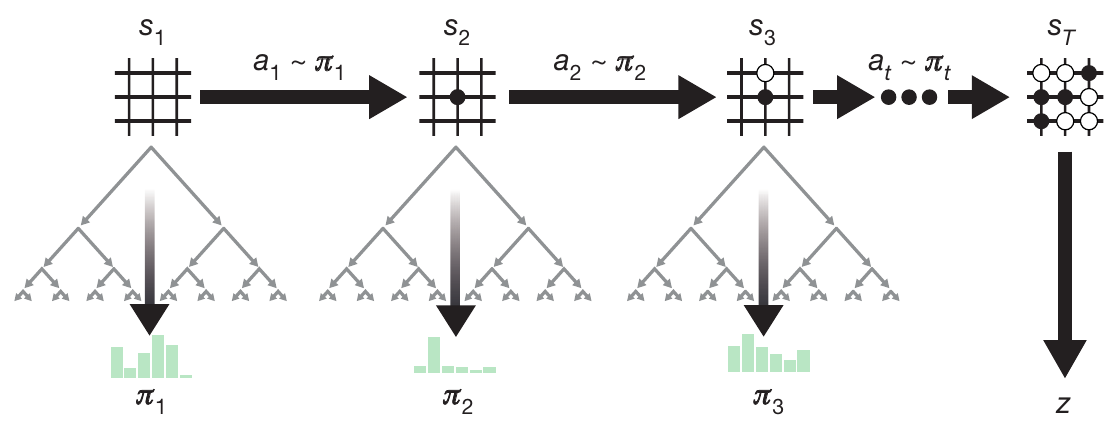
\includegraphics[width=\linewidth]{img/selfplay.png}
  \centering 
  \caption{Self play performed by AlphaGo Zero depicted in \citet{silver_mastering_2017}}
  \label{fig:selfplay}
\end{figure}

What follows is the second step of neural network \emph{(re)training}, illustrated in Figure \ref{fig:retraining}. From the previous iterations of self play, training data $(s_t,\pi_t,z_t)$ is sampled uniformly to re-train the network in order to more closely approximate the results of the MCTS. The loss is hereby made up of mean squared error for the estimated value, cross entropy for the predicted probability and L2-regularisation for the parameters $\theta$:

$$(z-v)^2 - \pi^T log p + c ||\theta||^2= L$$

\begin{figure}
  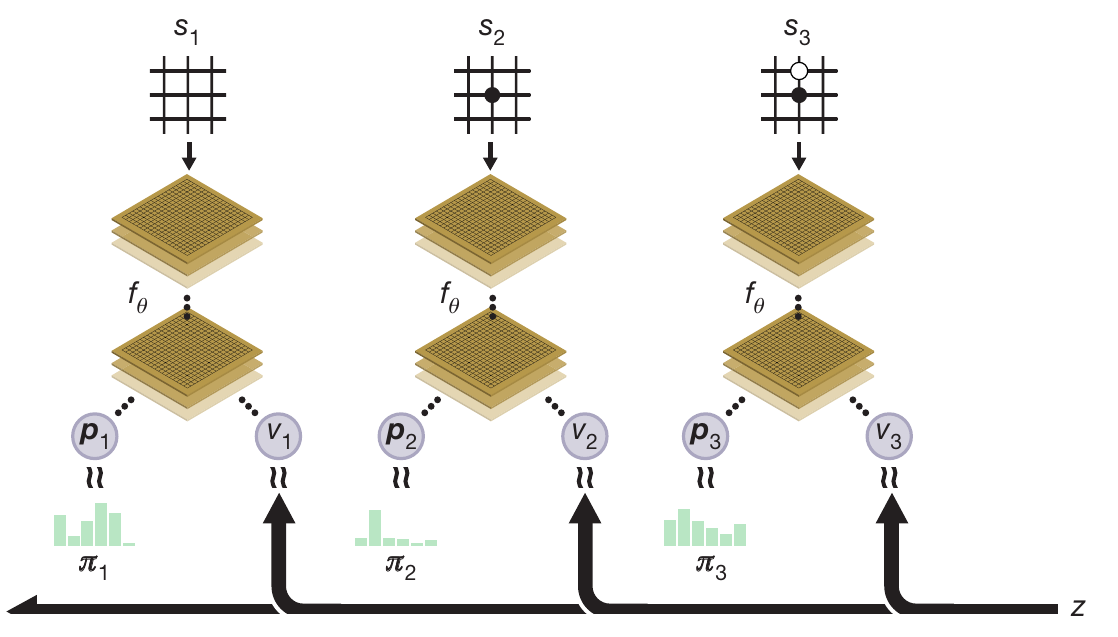
\includegraphics[width=12cm]{img/training.png}
  \centering 
  \caption{Model (re-)training in AlphaGo Zero as depicted in \citet{silver_mastering_2017}}
  \label{fig:retraining}
\end{figure}

During the last step of model evaluation, both the original and the retrained model play a number of games against each other using $f_\theta$ guided MCTS. The model that wins the majority of games is used in the next iteration. This way, the model $f_\theta$ is continuously improving and representing more and more of the optimal policy as approximated by the MCTS.

The final AlphaGo Zero model brought forth by \citet{silver_mastering_2017} consisted of 20 residual blocks and was trained for approximately 3 days with 4.9 million games using 1,600 simulations for each MCTS. It outperformed both previous networks after 36 and 73 hours of training respectively. 

\subsubsection{Specific implementation}
We borrowed the broad strokes of the algorithm described above for our model but still deviated from the original AlphaGo Zero model in a few relevant aspects: we did not use the history of the states as input and instead of a convolutional neural network with 20 residual blocks, we used a 30-120-30-120-(21,1) deep neural network with 3 hidden layers predicting given a state the probabilities for each action and the value. We ran 100 episodes with 500 MCTS simulation each, using 150 iterations of self-play with 1000 epochs and 200 games for model evaluation. This configuration was run twice in two different modes: The first mode was penalised, which means that during the evaluation, if the highest predicted probability did not correspond to a legal move, the current match will be lost. The non-penalised mode on the other hand would consider the highest probability restricted to the legal actions and pick a random legal action in case all legal actions where predicted with 0. Each configuration took roughly 2 days to finish running on our personal hardware.

\subsubsection{Benchmarking and Results}
For benchmarking we would let each new network (every time the model evaluation would lead to the new network win) play the same 1000 games against a random player that were also used for benchmarking the DQN approach. The results can be observed in Figure \ref{fig:alphazero}.

\begin{figure}
  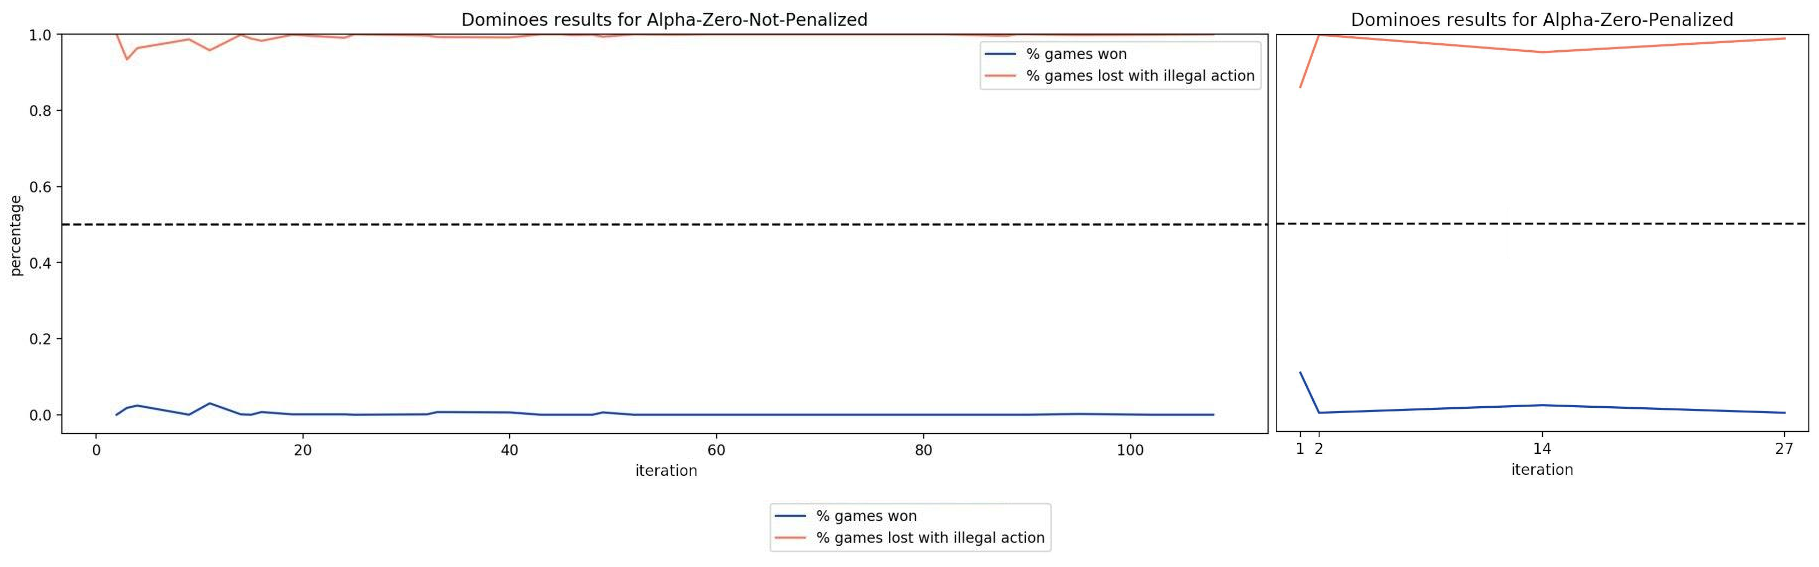
\includegraphics[width=\linewidth]{img/alphazero.png}
  \centering 
  \caption{Benchmarking results for AlphaGo Zero agents trained with and without penalisation of invalid moves. Benchmarking was performed every time the retrained model replaced the previous model.}
  \label{fig:alphazero}
\end{figure}

It becomes apparent from a first glance that these results are also rather disappointing. Both agents win basically no games and instead lose nearly every game. The non-penalised model starts promising but eventually also regresses. The poor performance of both models might be due to the fact that they learn a specific path from a specific set of starting states used during training which does not generalise well for other starting states. This could be solved by tweaking the exploration factor. However, we cannot be sure and the above results give little information on possible areas of improvement.

\subsubsection{Discussion}
As the third and last approach trying to find a model that would learn dominoes failed, we have to critically evaluate our methodology in order to find possible explanations for the poor behaviour, even when using state of the arts methods like AlphaGo Zero. One reason could be our deviations from the original model with a simpler architecture and without representing the game history in the encoding. This leads towards a broader point about the game encoding used throughout the project. It does not include the information about the order in which the different tiles formed the chain and the corresponding stacks. In the future this could be expanded to represent the environment’s states in more detail.
Another factor that might have hindered learning was the use of varying initial states. This most likely massively increased the learning difficulty as it confronted the agent with the task of generalisation even before learning concrete relationships. This probably massively hindered the agents' understanding of basic game mechanics (and probably also held back the DQN from surpassing a random player). 


\section{Conclusion}
While we did not accomplish the project goal, we learned a lot about supervised and reinforcement learning as well as machine learning architectures in general. While some approaches tested in this project are definitely promising and could potentially be used effectively after a little more fine-tuning, we were mostly held back by the time it took us to find a promising approach. Instead of sticking with one and really immersing ourselves, we chose to try multiple approaches hoping that one would deliver the expected results. This was not the case, partly because we were limited by our personal hardware and thus training time but also because we made some decisions early on in the project that most likely negatively affected all approaches. They include but are not limited to training with a random initial state, a game encoding that does not represent the game’s history, and a model architecture that was not sophisticated enough to represent relationships as complicated as the rules and strategies needed to win a game of dominoes.
However, our project was everything but pointless. What remains is a functioning framework for learning any kind of ASP-encodable game with any kind of implementable machine learning approach\footnote{The open source code for the project can be found in\\ \url{https://github.com/susuhahnml/asp-game-ml-strategies}}. We used it to apply the same approaches to the much simpler game Nim, the results of which are shown in Figure 15. We used the framework to generate visualisations for the game that show that at least for a simple fixed starting state all approaches manage to learn a winning strategy. In the future it would surely be promising to refine the framework by considering more behaviours from the original AlphaGo Zero or to use it to examine the effects of different game encodings and model architectures for the given approaches.

\begin{figure}
  \centering
\begin{subfigure}{\textwidth}
  \centering
  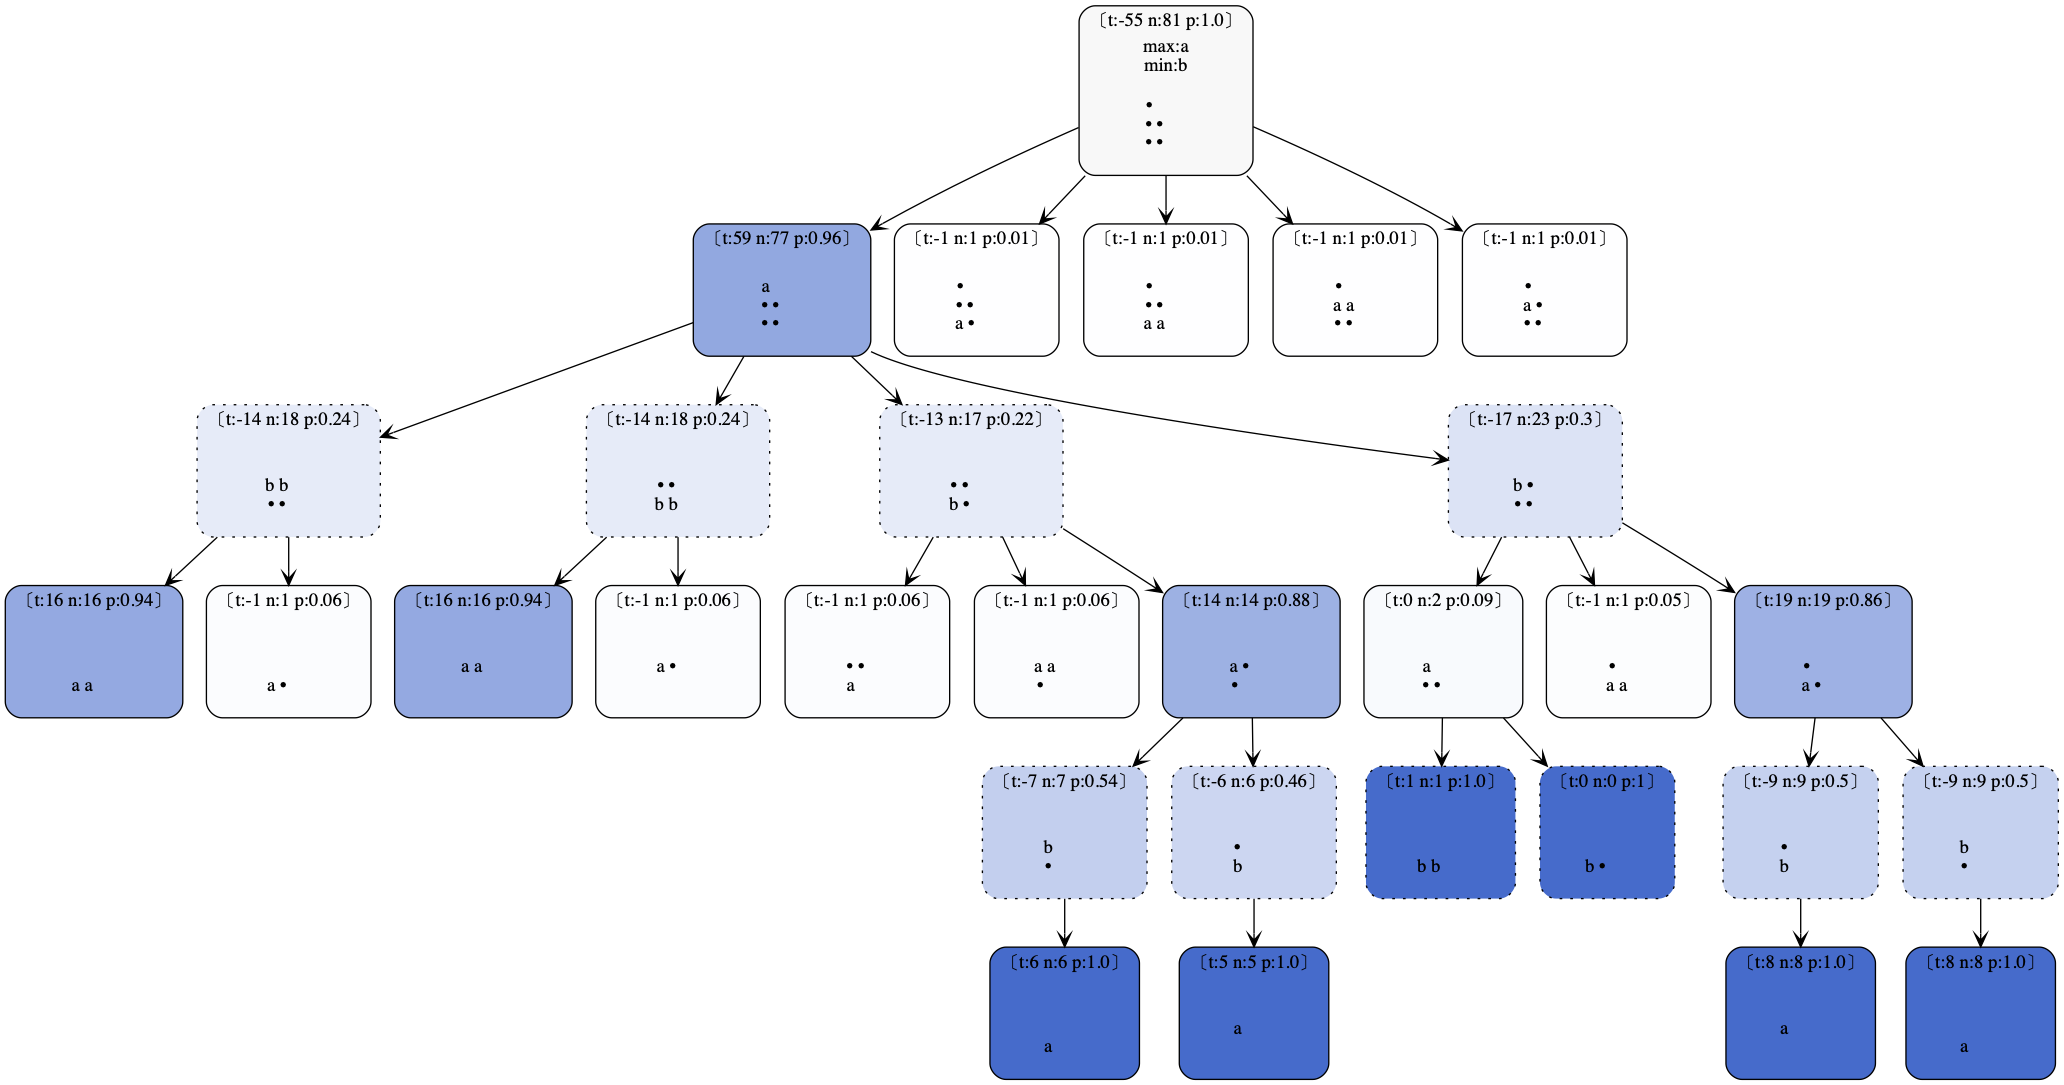
\includegraphics[width=\linewidth]{img/nim-mcts.png}
  \centering 
  \caption{Generated using my the MCTS algorithm, reaching early stopping after 81 iterations.}
\end{subfigure}%
\hspace{10px}
\begin{subfigure}{.45\textwidth}
  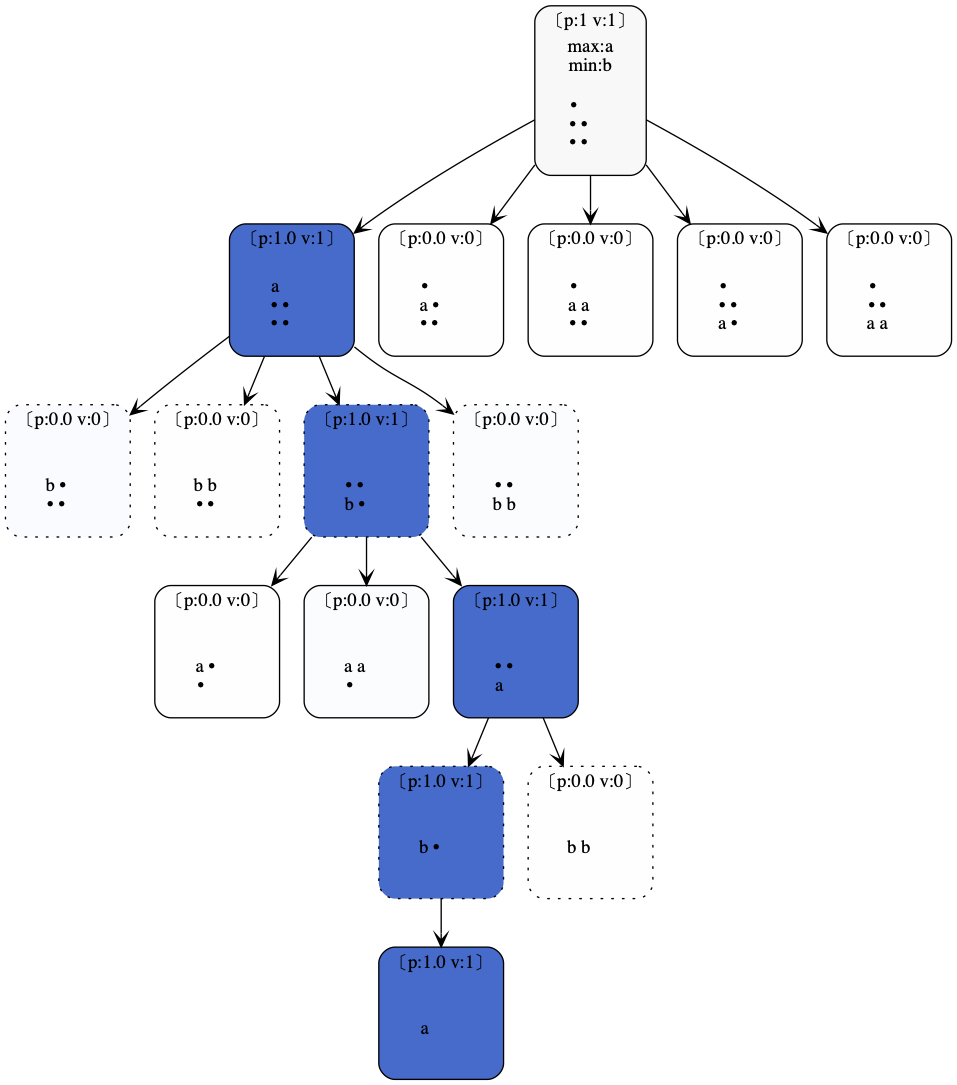
\includegraphics[width=0.9\linewidth]{img/nim-rl.png}
  \centering 
  \caption{Generated using the probabilities predicted by the our DQN approach.}
\end{subfigure}
\begin{subfigure}{.5\textwidth}
  \centering
  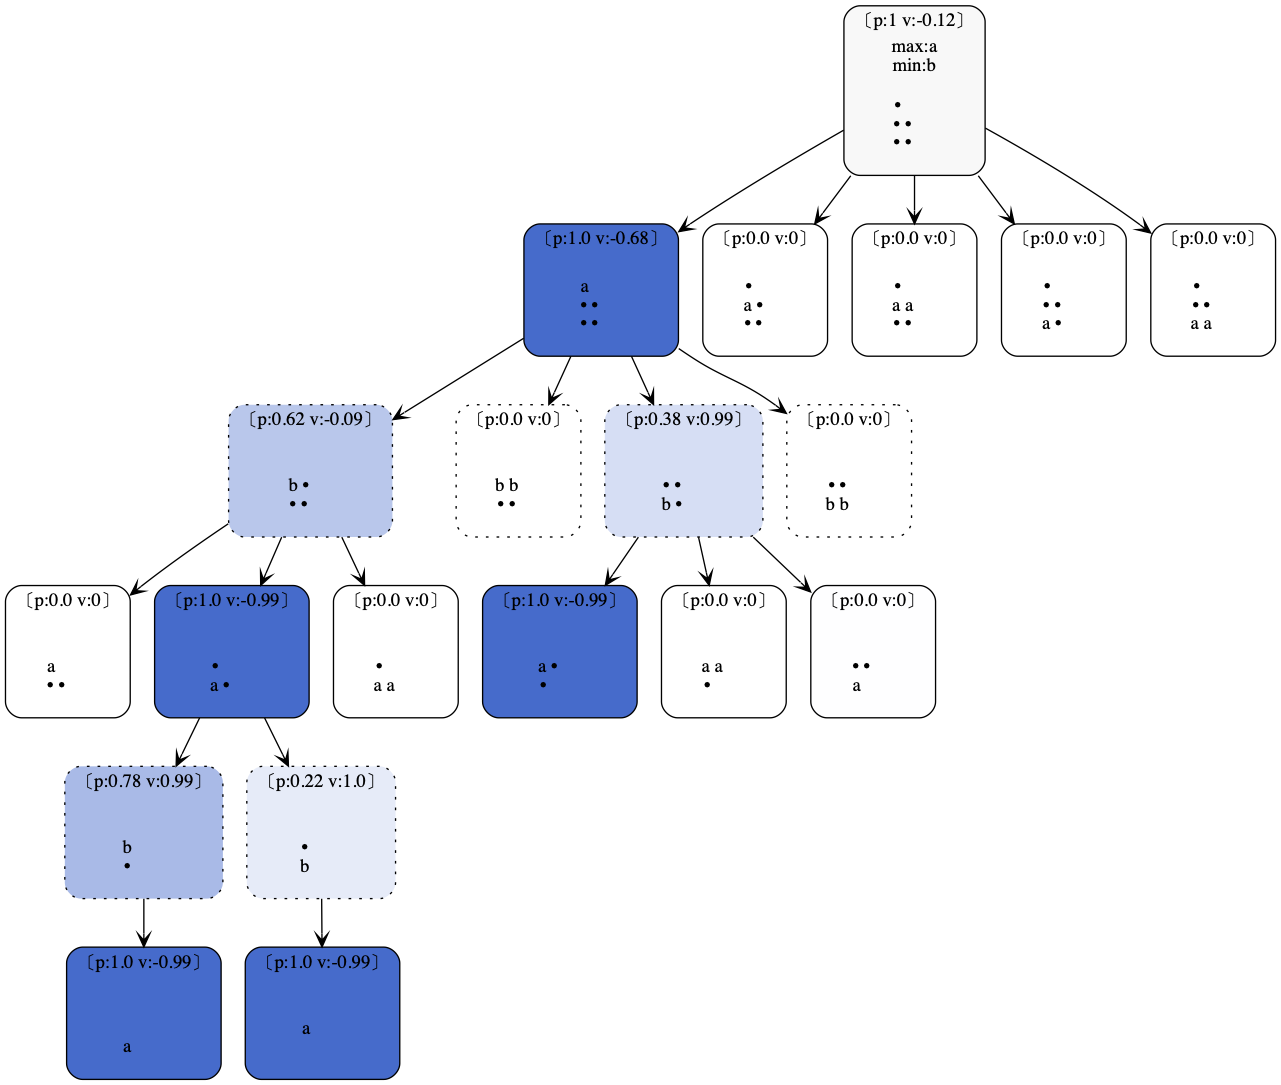
\includegraphics[width=\linewidth]{img/nim-alpha-zero.png}
  \caption{Generated using the probabilities predicted by the our AlphaZero approach.}
\end{subfigure}
\caption{Games trees generated for the game of Nim with a small initial state. Darker blue corresponds to moves with higher probability according to the network. States are not expanded if already present on the tree or if their probability is close to 0.}
\end{figure}



\addcontentsline{toc}{section}{References}
\bibliographystyle{apalike}
\bibliography{domiknows}

\appendix
\section{Rules for Nim}
\label{a:nimrules}
The game is usually played by two players.  \\
Both players alternately remove objects from distinct piles. \\
Each turn any number of objects can be removed from a pile as long as at least one object is removed. \\
Depending on the version being played, the goal of the game is either to avoid taking the last object, or to take the last object. \\ 
\\
The game is commonly played with match sticks with 4 piles consisting of 1, 3, 5, and 7 match sticks respectively.


\section{Rules for Two-Player Dominoes without a draw pile}
\label{a:domrules}
The game is played by two players. \\
Both players receive the same amount of dominoes. \\
One player starts by placing a domino on the board. \\
The other player has to put down a domino on either side of the first domino, matching the number on one side of the domino with one of the numbers on their domino. This creates a chain of dominoes. \\
The players now alternatively have to place their dominoes on either side of the chain, always matching the number on one side of the chain with one of the numbers on the domino they place. \\
If a player cannot put down a domino, they have to pass. \\
The player who first puts down all their dominoes wins.

\end{document}